\begin{frame}
    \frametitle{Model for urban traffic network}
    \metroset{block=fill}
    \begin{block}{Demand \& Supply paradigm}
    For a road $r$ we define
    \begin{itemize}
    \item Demand of $r$ the flow of vehicles that can go out from $r$
    \item Supply of $r$ the flow of vehicles that $r$ can receive
    \end{itemize}
    \end{block}
    \begin{center}
    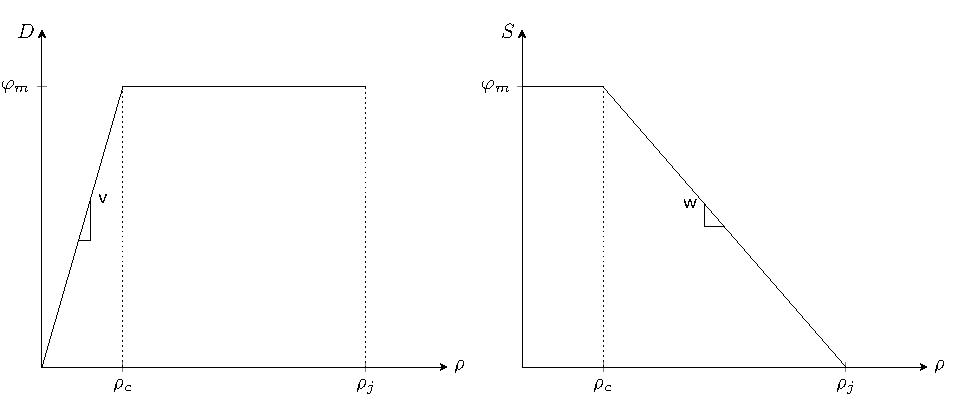
\includegraphics[scale=0.6]{fig_49_D-S}
    \end{center}
    \[
    D_r = \min \{ v\rho_r, \varphi_m\}
    \qquad
    S_r = \min\{ w(\rho_j-\rho) , \varphi_m \}
    \]
\end{frame}
